\documentclass{article}
\usepackage[utf8]{inputenc}
\usepackage{amsmath}
\usepackage{graphicx}
\usepackage{geometry}
\usepackage{hyperref}
\usepackage{tikz}
\usepackage{booktabs} % For professional-looking tables

% TikZ libraries for drawing
\usetikzlibrary{shapes.geometric, arrows, positioning, fit, calc}

\geometry{
    a4paper,
    left=2.5cm,
    right=2.5cm,
    top=2.5cm,
    bottom=2.5cm,
}

\title{Progress Report: A Two-Stage System for Real-Time Thai Profanity Detection and Censoring}
\date{\today}

\begin{document}

\maketitle

\section{Introduction}

The objective of this research is to develop a robust and accurate system for the detection and subsequent censoring of profane words in Thai audio streams. The primary challenge lies not only in accurately identifying spoken profanity but also in applying censorship in a way that is precise and minimally disruptive to the listening experience. This report outlines the methodologies explored, the development of a functional two-stage censoring system, key findings, and the direction for future work.

\section{Methodology}

Our approach has evolved from a foundational model to a more sophisticated, real-time pipeline. The core components of the methodology are detailed below.

\subsection{Core Detection Model: Fine-Tuned Wav2Vec2}

The primary model is based on \textbf{Wav2Vec2}, a powerful pre-trained architecture for speech representation. We employed a transfer learning approach by fine-tuning the \texttt{facebook/wav2vec2-base} model on a custom-labeled dataset of Thai profanity.

Key techniques used during training include:
\begin{itemize}
    \item \textbf{Data Preprocessing:} Audio segments were processed with a pre-emphasis filter to boost high-frequency components and a Hamming window to reduce signal leakage.
    \item \textbf{Data Augmentation:} To combat overfitting and improve model generalization, several augmentation techniques were applied, including random noise injection, time stretching, and pitch shifting.
    \item \textbf{Class Imbalance Handling:} A weighted loss function was implemented to assign higher importance to the under-represented profanity classes, ensuring the model learns to detect rare words effectively.
\end{itemize}

We also established a framework (\texttt{advanced\_model\_training.py}) to experiment with alternative architectures like CNN-LSTM and Transformers, though Wav2Vec2 remains the current production model.

\subsection{Model Architecture and Training Comparison}

To push the performance beyond the baseline, we developed two distinct training pipelines.

\subsubsection{Baseline: Fine-Tuned Wav2Vec2}
The initial approach, encapsulated in \texttt{fine\_tune\_wav2vec2\_sen\_ham\_CW.py}, relies on the standard Hugging Face \texttt{Trainer} API. It fine-tunes a pre-trained Wav2Vec2 model and incorporates essential techniques such as applying a Hamming window, using a pre-emphasis filter, and implementing a custom trainer with class weights to handle data imbalance. This script provides a strong and reliable baseline for profanity detection.

\subsubsection{Advanced Framework: Experimental Architectures}
The second pipeline, \texttt{advanced\_model\_training.py}, is a more sophisticated framework built with PyTorch for rapid experimentation. Its key advantages include:
\begin{itemize}
    \item \textbf{Architectural Flexibility:} It supports multiple model types, including an enhanced Wav2Vec2, custom Transformers, and the CNN-LSTM hybrid model diagrammed in Figure \ref{fig:cnn-lstm-arch}.
    \item \textbf{Advanced Augmentation:} It introduces a wider array of data augmentation techniques, such as SpecAugment, noise injection, time stretching, and pitch shifting, for creating a more robust model.
    \item \textbf{Rigorous Evaluation:} The framework is designed for k-fold cross-validation, allowing for more reliable and generalizable performance metrics.
\end{itemize}

\begin{table}[h!]
\centering
\caption{Comparison of Training Script Features}
\label{tab:script-comparison}
\resizebox{\textwidth}{!}{
\begin{tabular}{@{}lll@{}}
\toprule
\textbf{Feature} & \textbf{Baseline Script (fine\_tune\_...)} & \textbf{Advanced Framework (advanced\_...)} \\
\midrule
Framework & Hugging Face Trainer & PyTorch Custom Loop + Hugging Face Trainer \\
Supported Models & Wav2Vec2 & Wav2Vec2, CNN-LSTM, Transformer \\
Preprocessing & Pre-emphasis, Hamming Window & Spectral Subtraction, Normalization, etc. \\
Augmentation & Basic (Noise, Pitch, Speed) & Advanced (SpecAugment, Mixup, etc.) \\
Imbalance Handling & Weighted Loss & Weighted Loss \& Weighted Random Sampler \\
Evaluation & Train/Val Split, K-Fold & Stratified K-Fold, Detailed Reports \\
Configurability & Hardcoded Parameters & Config File \& Command-Line Args \\
\bottomrule
\end{tabular}
}
\end{table}

\begin{figure}[h!]
\centering
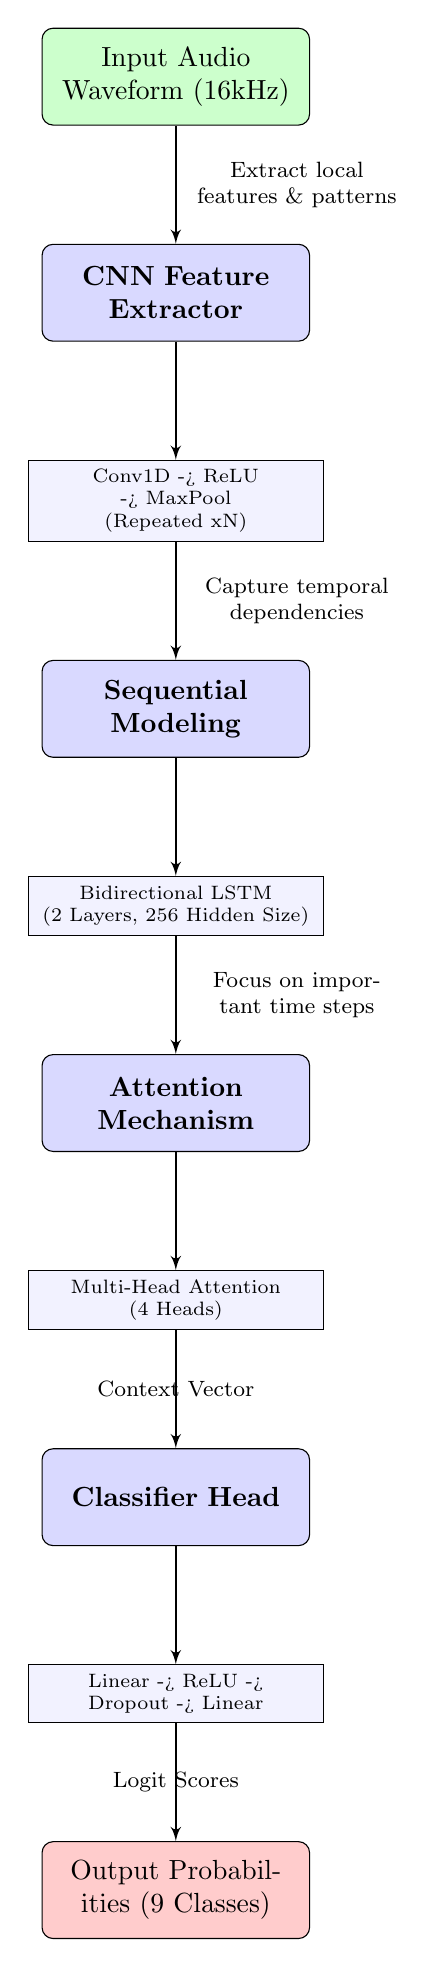
\begin{tikzpicture} [
    node distance=1.5cm and 0.5cm,
    block/.style={rectangle, draw, fill=blue!15, text width=9em, text centered, rounded corners, minimum height=3.5em},
    small_block/.style={rectangle, draw, fill=blue!5, text width=10em, text centered, minimum height=2em, font=\scriptsize},
    line/.style={draw, -latex', thick},
    anno/.style={text width=8em, text centered, font=\footnotesize, midway}
]
    % Nodes
    \node[block, fill=green!20] (input) {Input Audio Waveform (16kHz)};

    \node[block, below=of input] (cnn) {\textbf{CNN Feature Extractor}};
    \node[small_block, below=of cnn, node distance=1.2cm] (cnn_details) {Conv1D -¿ ReLU -¿ MaxPool \\ (Repeated xN)};

    \node[block, below=of cnn_details, node distance=1.8cm] (lstm) {\textbf{Sequential Modeling}};
    \node[small_block, below=of lstm, node distance=1.2cm] (lstm_details) {Bidirectional LSTM \\ (2 Layers, 256 Hidden Size)};

    \node[block, below=of lstm_details, node distance=1.8cm] (attention) {\textbf{Attention Mechanism}};
    \node[small_block, below=of attention, node distance=1.2cm] (attention_details) {Multi-Head Attention \\ (4 Heads)};

    \node[block, below=of attention_details, node distance=1.8cm] (classifier) {\textbf{Classifier Head}};
    \node[small_block, below=of classifier, node distance=1.2cm] (classifier_details) {Linear -¿ ReLU -¿ Dropout -¿ Linear};

    \node[block, fill=red!20, below=of classifier_details, node distance=2cm] (output) {Output Probabilities (9 Classes)};

    % Arrows with Annotations
    \path [line] (input) -- node[anno, right] {Extract local features \& patterns} (cnn);
    \path [line] (cnn) -- (cnn_details);
    \path [line] (cnn_details) -- node[anno, right] {Capture temporal dependencies} (lstm);
    \path [line] (lstm) -- (lstm_details);
    \path [line] (lstm_details) -- node[anno, right] {Focus on important time steps} (attention);
    \path [line] (attention) -- (attention_details);
    \path [line] (attention_details) -- node[anno] {Context Vector} (classifier);
    \path [line] (classifier) -- (classifier_details);
    \path [line] (classifier_details) -- node[anno] {Logit Scores} (output);

\end{tikzpicture}
\caption{Architecture of the Experimental CNN-LSTM Model, detailing the flow from raw audio to classification.}
\label{fig:cnn-lstm-arch}
\end{figure}

\subsection{Model Architecture Comparison}

To identify the most effective approach for this task, we are comparing two distinct model architectures: a fine-tuned Transformer-based model (Wav2Vec2) and a custom-built hybrid model (CNN-LSTM).

\subsubsection{Baseline Model: Fine-Tuned Wav2Vec2}
Our baseline is the \textbf{Wav2Vec2} model. This is a state-of-the-art architecture pre-trained on thousands of hours of unlabeled audio data. At its core, it uses a multi-layer Transformer to process the raw audio waveform directly, learning powerful and general-purpose representations of speech. For our task, we keep the pre-trained model frozen and only fine-tune a new classification head on top. Its primary strength is its ability to understand speech context from raw audio without needing intermediate representations like spectrograms.

\subsubsection{Experimental Model: CNN-LSTM Hybrid}
As an alternative, we designed a hybrid architecture, illustrated in Figure \ref{fig:cnn-lstm-arch}, that combines two classical deep learning components for audio processing:
\begin{itemize}
    \item \textbf{1D CNN Layers:} The initial layers are a series of 1D Convolutional Neural Networks. These act as a trainable feature extractor, scanning the raw audio to identify low-level local patterns like phonemes, onsets, and specific sound textures.
    \item \textbf{Bidirectional LSTM Layers:} The sequence of features extracted by the CNN is then fed into a Bidirectional Long Short-Term Memory network. The LSTM's role is to model the temporal dependencies in the sequence, learning how sounds evolve over time. Its bidirectionality allows it to use both past and future context to make a more informed decision at each time step.
    \item \textbf{Attention Mechanism:} A multi-head attention layer is applied to the LSTM output. This allows the model to dynamically weigh the importance of different parts of the audio sequence, focusing only on the segments most indicative of profanity before making a final decision.
\end{itemize}
This custom-built model allows for more granular control over the architecture and is designed to be a more lightweight alternative to the large Transformer-based Wav2Vec2.

\section{Results and Key Findings}

Through the implementation of the aforementioned systems, we have arrived at several key findings:

\begin{enumerate}
    \item \textbf{Initial Model Performance:} The initial fine-tuned Wav2Vec2 model demonstrated high accuracy on the validation dataset but suffered from slight overfitting and imprecise real-world application when using a simple windowing method.
    
    \item \textbf{Failure of Simple Windowing:} Censoring the entire 0.5-second window for every detection was functionally correct but resulted in a poor user experience. It often censored significant portions of non-profane speech and was highly disruptive.
    
    \item \textbf{Success of the Two-Stage System:} The “Detect, then Refine” pipeline proved significantly more effective. The output from this system is far less intrusive, with censorship being applied only to the spoken profane word. This is a major step towards a production-ready system.
    
    \item \textbf{System Debugging:} During testing of the frame-level system, we identified and resolved two critical bugs:
    \begin{itemize}
        \item An issue where the model output generic \texttt{LABEL\_0} instead of the correct Thai labels. This was fixed by hardcoding the correct label map into the script.
        \item An overly aggressive window-merging algorithm that censored long periods of clean speech between two distant profane words. This was corrected by introducing a maximum gap parameter (\texttt{max\_merge\_gap}) to control the merging behavior.
    \end{itemize}
\end{enumerate}

\begin{table}[h!]
\centering
\caption{Preliminary Model Performance Comparison}
\label{tab:model-comparison}
\begin{tabular}{@{}lccccc@{}}
\toprule
Model & Accuracy & Binary Acc. & Precision & Recall & F1-Score \\
\midrule
Baseline Wav2Vec2 & 30.5\% & 63.5\% & 67.1\% & 30.6\% & 41.9\% \\
Advanced CNN-LSTM & 26.3\% & 55.2\% & 50.1\% & 24.1\% & 34.2\% \\
\bottomrule
\end{tabular}
\end{table}

\begin{figure}[h!]
\centering
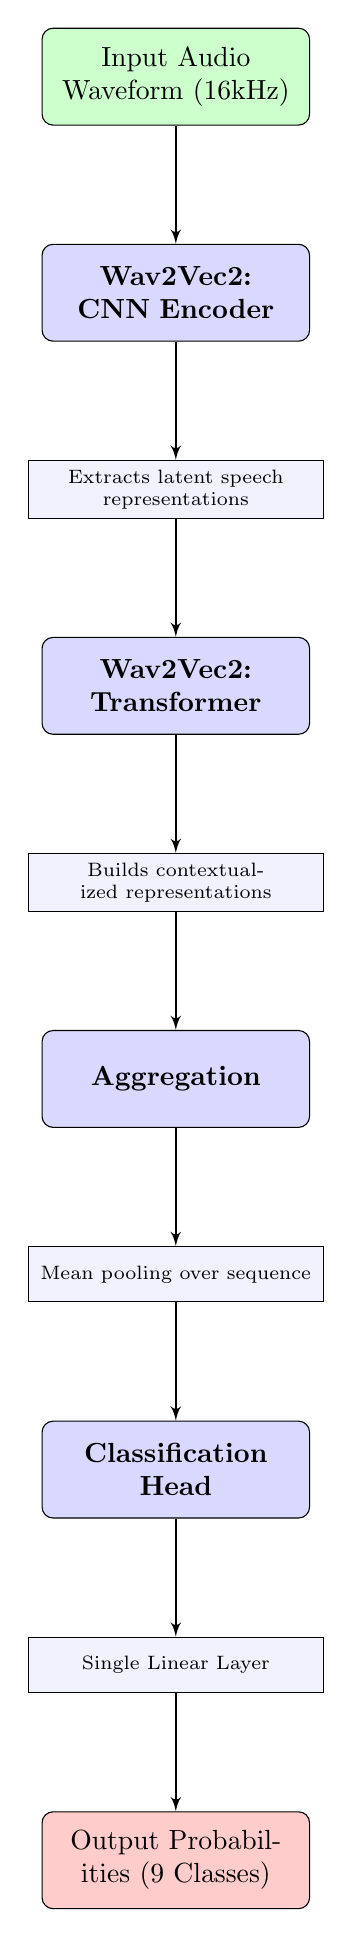
\begin{tikzpicture} [
    node distance=1.5cm and 0.5cm,
    block/.style={rectangle, draw, fill=blue!15, text width=9em, text centered, rounded corners, minimum height=3.5em},
    small_block/.style={rectangle, draw, fill=blue!5, text width=10em, text centered, minimum height=2em, font=\scriptsize},
    line/.style={draw, -latex', thick},
    anno/.style={text width=8em, text centered, font=\footnotesize, midway}
]
    % Nodes
    \node[block, fill=green!20] (input) {Input Audio Waveform (16kHz)};
    \node[block, below=of input] (feature_encoder) {\textbf{Wav2Vec2: CNN Encoder}};
    \node[small_block, below=of feature_encoder, node distance=1.2cm] (feature_encoder_details) {Extracts latent speech representations};

    \node[block, below=of feature_encoder_details, node distance=1.8cm] (transformer) {\textbf{Wav2Vec2: Transformer}};
    \node[small_block, below=of transformer, node distance=1.2cm] (transformer_details) {Builds contextualized representations};

    \node[block, below=of transformer_details, node distance=1.8cm] (pooling) {\textbf{Aggregation}};
    \node[small_block, below=of pooling, node distance=1.2cm] (pooling_details) {Mean pooling over sequence};

    \node[block, below=of pooling_details, node distance=1.8cm] (classifier) {\textbf{Classification Head}};
    \node[small_block, below=of classifier, node distance=1.2cm] (classifier_details) {Single Linear Layer};

    \node[block, fill=red!20, below=of classifier_details, node distance=2cm] (output) {Output Probabilities (9 Classes)};

    % Arrows
    \path [line] (input) -- (feature_encoder);
    \path [line] (feature_encoder) -- (feature_encoder_details);
    \path [line] (feature_encoder_details) -- (transformer);
    \path [line] (transformer) -- (transformer_details);
    \path [line] (transformer_details) -- (pooling);
    \path [line] (pooling) -- (pooling_details);
    \path [line] (pooling_details) -- (classifier);
    \path [line] (classifier) -- (classifier_details);
    \path [line] (classifier_details) -- (output);

\end{tikzpicture}
\caption{Architecture of the Baseline Fine-Tuned Wav2Vec2 Model.}
\label{fig:wav2vec2-arch}
\end{figure}

\section{Future Work}

While the current system is a robust proof-of-concept, the following steps are planned to further improve and validate its performance:

\begin{itemize}
    \item \textbf{Quantitative Frame-Level Evaluation:} Create a "gold standard" test set of full-length audio files with precise, manually-annotated start and end times for every profane word. This will allow us to calculate formal evaluation metrics like Precision, Recall, and F1-Score at the frame level, providing a true measure of the system's real-world accuracy.
    
    \item \textbf{Advanced Censoring Techniques:} Move beyond simple silencing. The precise boundaries from Stage 2 enable more sophisticated techniques like replacing the profanity with generated non-verbal sounds (audio infilling) or a simple beep.
    
    \item \textbf{Model Architecture Comparison:} Conduct a full cross-validation experiment using the \texttt{advanced\_model\_} \texttt{training.py} framework to formally compare the performance of the Wav2Vec2, CNN-LSTM, and Transformer models.

\end{itemize}

\end{document}
